\section{Схемы с доверенным центром}\label{key-distribution-schemas}\index{схема!распределения ключей!(}
\selectlanguage{russian}

Схемы распределения ключей с доверенным центром состоят из трёх этапов.

\begin{enumerate}
    \item На первом этапе доверенный центр создаёт некоторый секрет, известный только ему. Это может быть некоторая секретная матрица с особыми свойствами, как в схеме Блома из раздела~\ref{section-bloms-scheme}, или пара из закрытого и открытого ключей, как в схеме Жиро из раздела~\ref{section-girault-scheme}.
    \item Для каждого нового легального участника сети доверенный центр, используя свою секретную информацию, вырабатывает некоторый отпечаток или сертификат, который позволяет новому участнику вырабатывать сеансовые ключи с другими легальными участниками.
    \item Наконец, на третьем этапе, когда начинается протокол общения двух легальных участников, они предъявляют друг-другу идентификаторы и/или дополнительную информацию от доверенного центра. Используя её, без дополнительного обращения к центру, они могут сгенерировать секретный сеансовый ключ для общения между собой.
\end{enumerate}

\subsection{Взаимная аутентификация с доверенным центром}
\selectlanguage{russian}

В \emph{протоколе Жиро}\index{протокол!Жиро} (\langfr{Marc Girault},~\cite{Girault:1990, Girault:1991}) участвуют три стороны -- $A$, $B$ и надёжный центр $T$.
\begin{enumerate}
    \item У стороны $T$ есть открытый и закрытый ключи криптосистемы RSA\index{криптосистема!RSA},
        \[ n=pq, ~ e, ~ d=e^{-1} \mod \varphi(n), \]
        с дополнительным параметром $g$ -- генератором подгруппы максимально возможного порядка мультипликативной группы $\Z_n^*$:
        \[ \begin{array}{l}
            \PK_T = (n, e, g) ~~\text{открытый ключ}, \\
            \SK_T = (d) ~~ \text{закрытый ключ}. \\
        \end{array} \]
    \item Стороны $A$ и $B$ независимо друг от друга создают свои открытые и закрытые ключи, обмениваясь информацией с центром $T$ по надёжному защищённому каналу. Стороны $A$ и $B$ выбирают свои закрытые ключи:
        \[ \begin{array}{l}
            \SK_A = a, \\
            \SK_B = b \\
        \end{array} \]
     и отправляют центру сообщения:
        \[ \begin{array}{ll}
            A \to T: & ~ I_A, ~~ g^{-\SK_A} = g^{-a} \mod n, \\
            B \to T: & ~ I_B, ~~ g^{-\SK_B} = g^{-b} \mod n, \\
        \end{array} \]
        где $I_A, I_B$ -- числовые идентификаторы сторон.
    \item Центр $T$ вычисляет открытые ключи для $A$ и $B$ и также по надёжному каналу передаёт им:
        \[ \begin{array}{ll}
            A \leftarrow T: & ~ \PK_A = (g^{-\SK_A} - I_A)^{\SK_T} = (g^{-a} - I_A)^d \mod n, \\
            B \leftarrow T: & ~ \PK_B = (g^{-\SK_B} - I_B)^{\SK_T} = (g^{-b} - I_B)^d \mod n. \\
        \end{array} \]
    \item Теперь стороны $A$ и $B$ могут создать общий секретный симметричный сеансовый ключ. Например, $A$ находит:
        \[ \begin{array}{ll}
            A: ~~ K_A & = ~ (\PK_B^e + I_B)^{\SK_A} ~ = \\
                & = ~ (((g^{-b} - I_B)^d)^e + I_B)^a ~ = \\
                & = ~ (g^{-b} - I_B + I_B)^a ~ = \\
                & = ~ g^{-ab} \mod n. \\
        \end{array} \]
        Аналогично $B$ вычисляет:
            \[ K_B = (\PK_A^e + I_A)^{\SK_B} = g^{-ab} \mod n. \]
        Как видно, ключи одинаковы:
            \[ K = K_A = K_B = g^{-ab} \mod n. \]
\end{enumerate}


\subsection{Схема Блома}\label{section-bloms-scheme}\index{схема!Блома|(}
\selectlanguage{russian}

Схема Блома (\langen{Rolf Blom},~\cite{Blom:1984, Blom:1985}) используется в протоколе HDCP\index{протокол!HDCP} (\langen{High-bandwidth Digital Content Protection}) для предотвращения копирования высококачественного видеосигнала. Предполагается, что некоторый доверенный центр распределит ключи таким образом, что легальные производители видеокарт, мониторов высокого разрешения и других компонент будут передавать видеоконтент по защищённому каналу, а <<пиратские>> устройства не смогут эти данные перехватить, и, например, записать на другой носитель.

На этапе инициализации доверенный центр выбирает симметричную матрицу $D_{m,m}$ над конечным полем $\GF p$. Для присоединения к сети распространения ключей, новый участник либо самостоятельно, либо с помощью доверенного центра выбирает новый открытый ключ (идентификатор) $I_i$, представляющий собой вектор длины $m$ над $\GF p$. Доверенный центр вычисляет для нового участника закрытый ключ $K_i$:
\begin{equation}
	K_i = D_{m,m} I_i.
	\label{eq:blom_center_matrix}
\end{equation}

Симметричность матрицы $D_{m,m}$ доверенного центра позволяет любым двум участникам сети создать общий сеансовый ключ. Пусть Алиса и Боб -- легальные пользователи сети, то есть они обладают открытыми ключами $I_A$ и $I_B$ соответственно, а их закрытые ключи $K_A$ и $K_B$ были вычислены одним и тем же доверенным центром по формуле~\ref{eq:blom_center_matrix}. Тогда протокол выработки общего секретного ключа выглядит следующим образом (рис.~\ref{fig:key_distribution-bloms-scheme}).

\begin{figure}
    \centering
    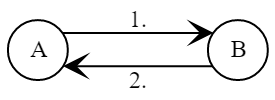
\includegraphics[width=0.5\textwidth]{pic/key_distribution-bloms-scheme}
    \caption{Взаимодействие участников в схеме Блома\label{fig:key_distribution-bloms-scheme}}
\end{figure}

\begin{protocol}
    \item[(1)] $Alice \to \left\{ I_A \right\} \to Bob$
    \item[(2)] Боб вычисляет $K_{BA} = K^T_B I_A = I^T_B D_{m,m} I_A$.
    \item[{}] $Bob \to \left\{ I_B \right\} \to Alice$
    \item[(3)] Алиса вычисляет $K_{AB} = K^T_A I_B = I^T_A D_{m,m} I_B$.
\end{protocol}

Из симметричности матрицы $D_{m,m}$ следует, что значения $K_{AB}$ и $K_{BA}$ совпадут, они же и будут являться общим секретным ключом для Алисы и Боба. Этот секретный ключ будет свой для каждой пары легальных пользователей сети.

Присоединение новых участников к схеме строго контролируется доверенным центром, что позволяет защитить сеть от нелегальных пользователей. Надёжность данной схемы основывается на невозможности восстановить исходную матрицу. Однако для восстановления матрицы доверенного центра размера $m \times m$ необходимо и достаточно всего $m$ пар линейно независимых открытых и закрытых ключей. В 2010-м году компания Intel, которая является <<доверенным центром>> для пользователей системы защиты HDCP, подтвердила, что криптоаналитикам удалось найти секретную матрицу (точнее, аналогичную ей), используемую для генерации ключей в упомянутой системе предотвращения копирования высококачественного видеосигнала.

\index{схема!Блома|)}

\index{схема!распределения ключей!)}